\section{Dataset}
We have collected several sequences with the sensor rig to showcase the potential of the system.
The current dataset consists of one sequence where we filmed an \gls{usv} from land, one where we filmed from a moving ship and a two other scenes where we walk around near the water.
The dataset contains the raw data from the cameras together with metadata for each frame, raw data from the \gls{imu} and raw data from the \gls{gnss} receivers.
A short sequence where we film a chess board while rotating the sensor rig is also included for calibration purposes.
More data will be collected and added to the dataset in the future.

The dataset is available at \url{TODO}.
Following is a selection of images from the dataset with the $S0$ image on the left, which is what a regular camera would capture, and the polarized image on the right.

\begin{figure}[H]
    \begin{subfigure}[T]{.49\textwidth}
        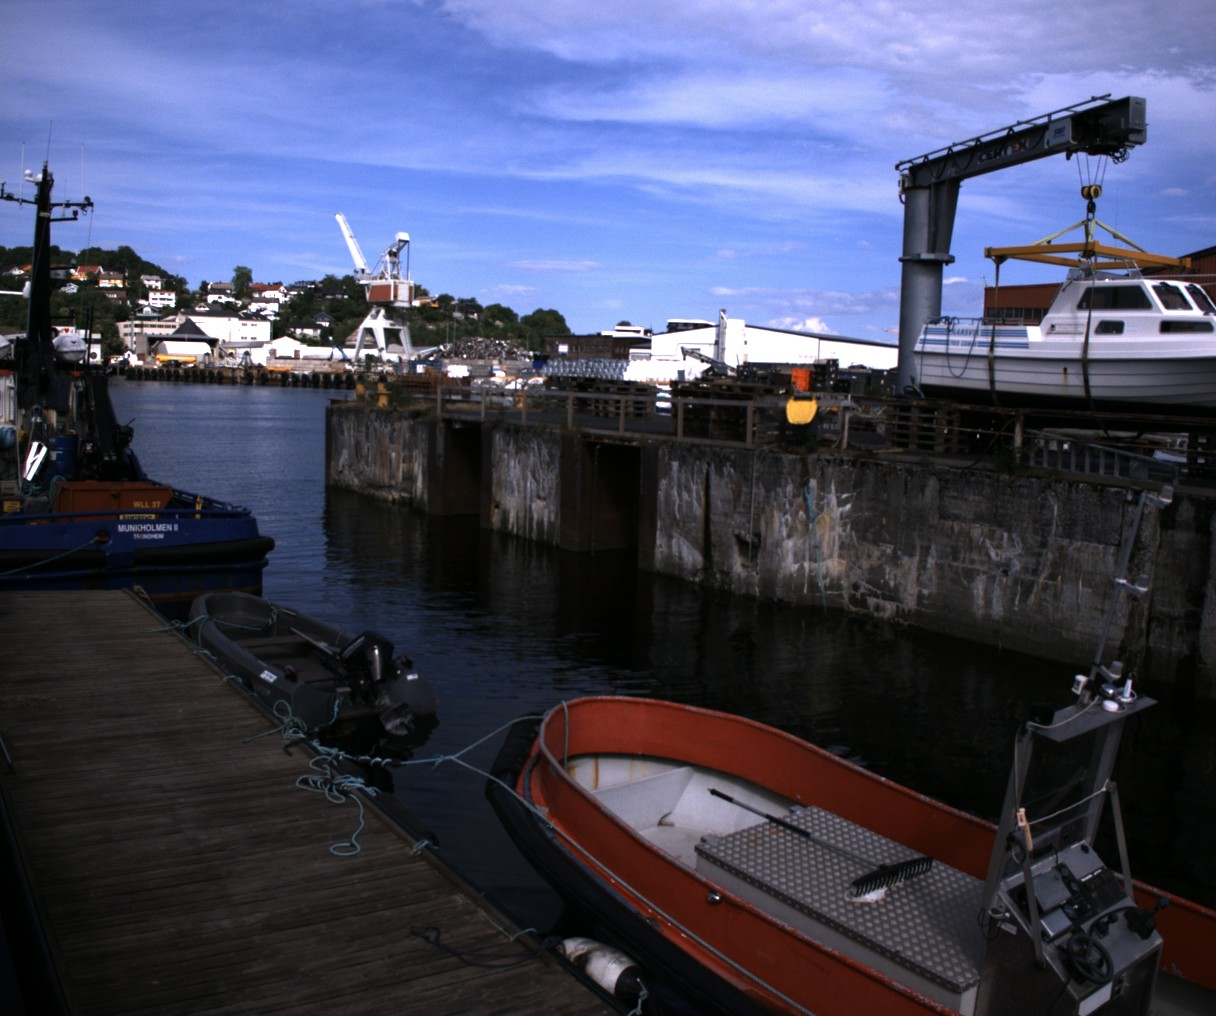
\includegraphics[width=\textwidth]{figures/pictures/img_2790_s0.jpg}
    \end{subfigure} \hfill
    \begin{subfigure}[T]{.49\textwidth}
        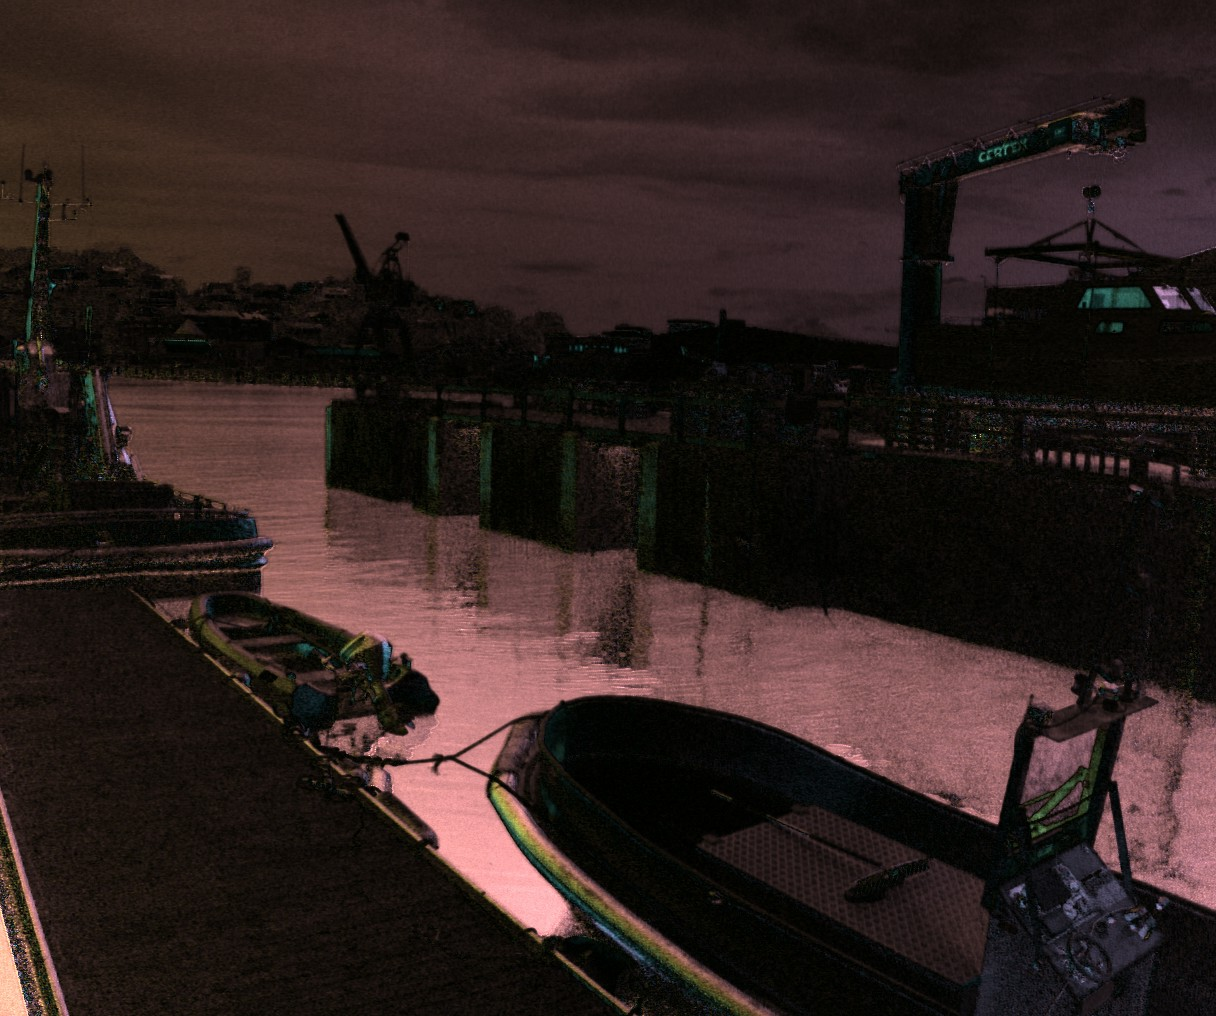
\includegraphics[width=\textwidth]{figures/pictures/img_2790_pol.jpg}
    \end{subfigure}
    \caption{Docking area.}
\end{figure}
\vspace{-.5cm}

\begin{figure}[H]
    \begin{subfigure}[T]{.49\textwidth}
        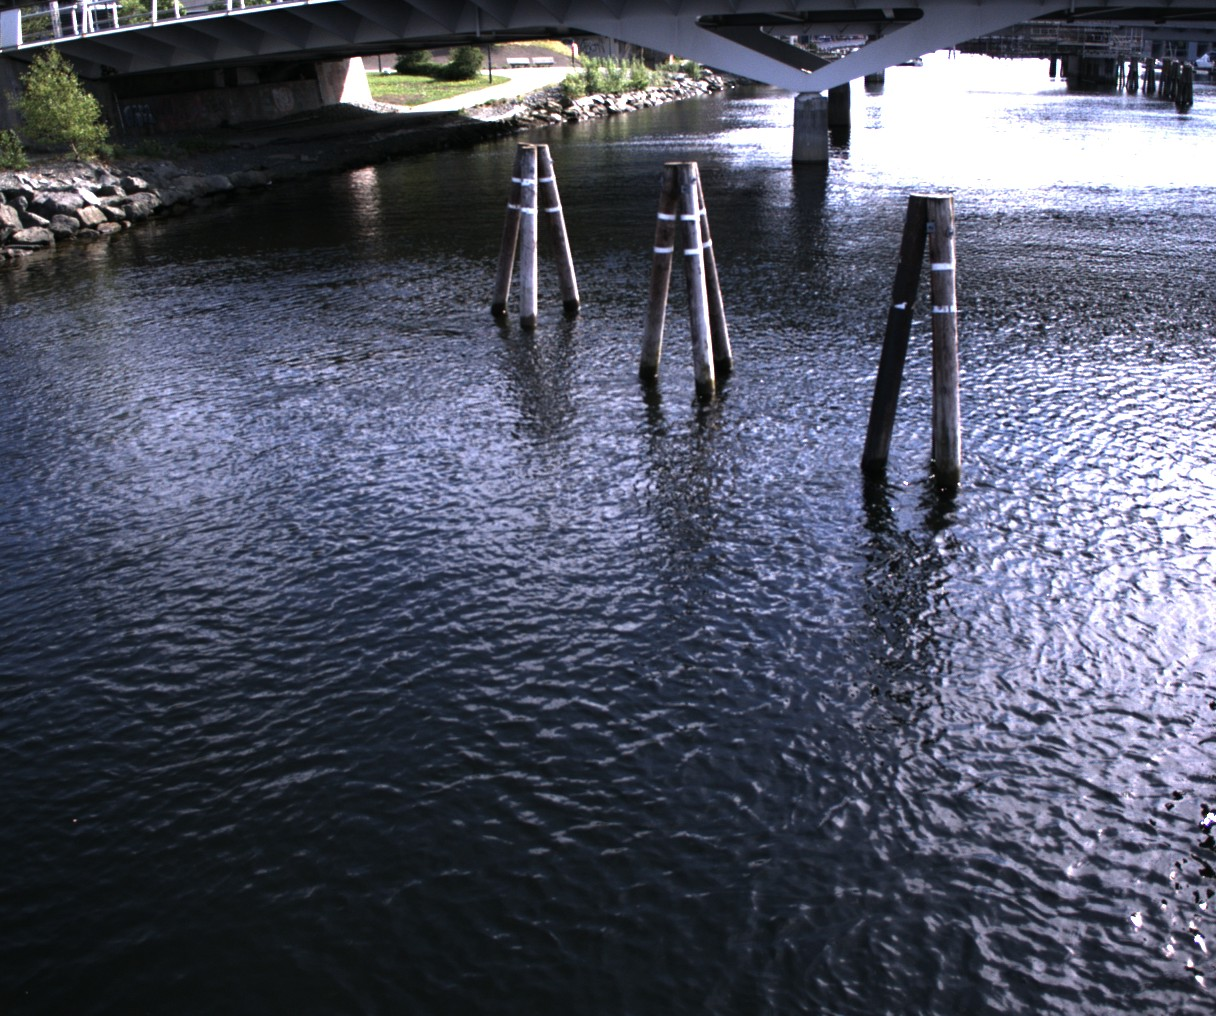
\includegraphics[width=\textwidth]{figures/pictures/img_7458_s0.jpg}
    \end{subfigure} \hfill
    \begin{subfigure}[T]{.49\textwidth}
        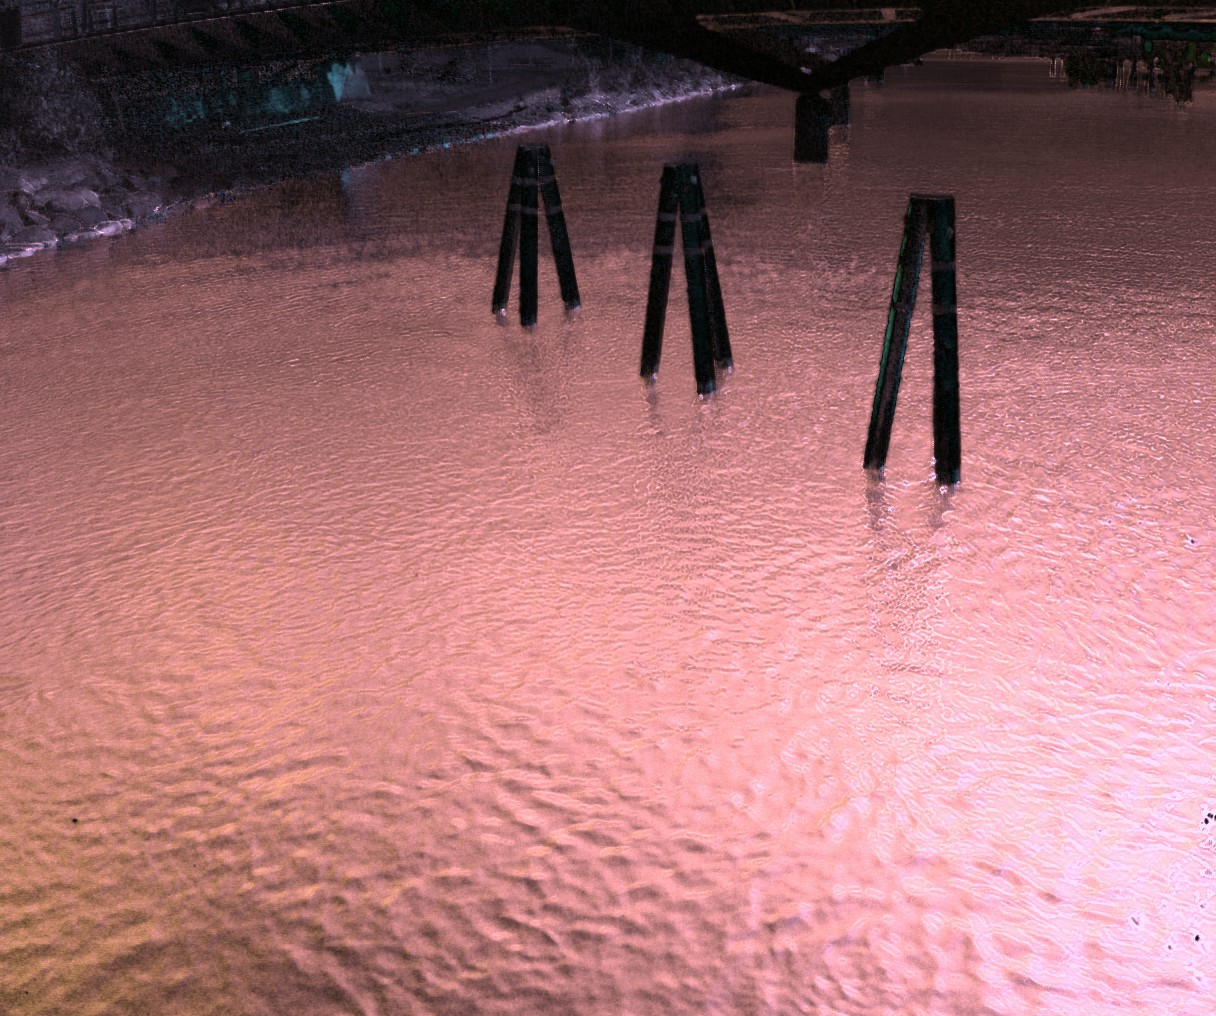
\includegraphics[width=\textwidth]{figures/pictures/img_7458_pol.jpg}
        
    \end{subfigure}
    \caption{Wooden posts in the water.}
\end{figure}
\vspace{-.5cm}

\begin{figure}[H]
    \begin{subfigure}[T]{.49\textwidth}
        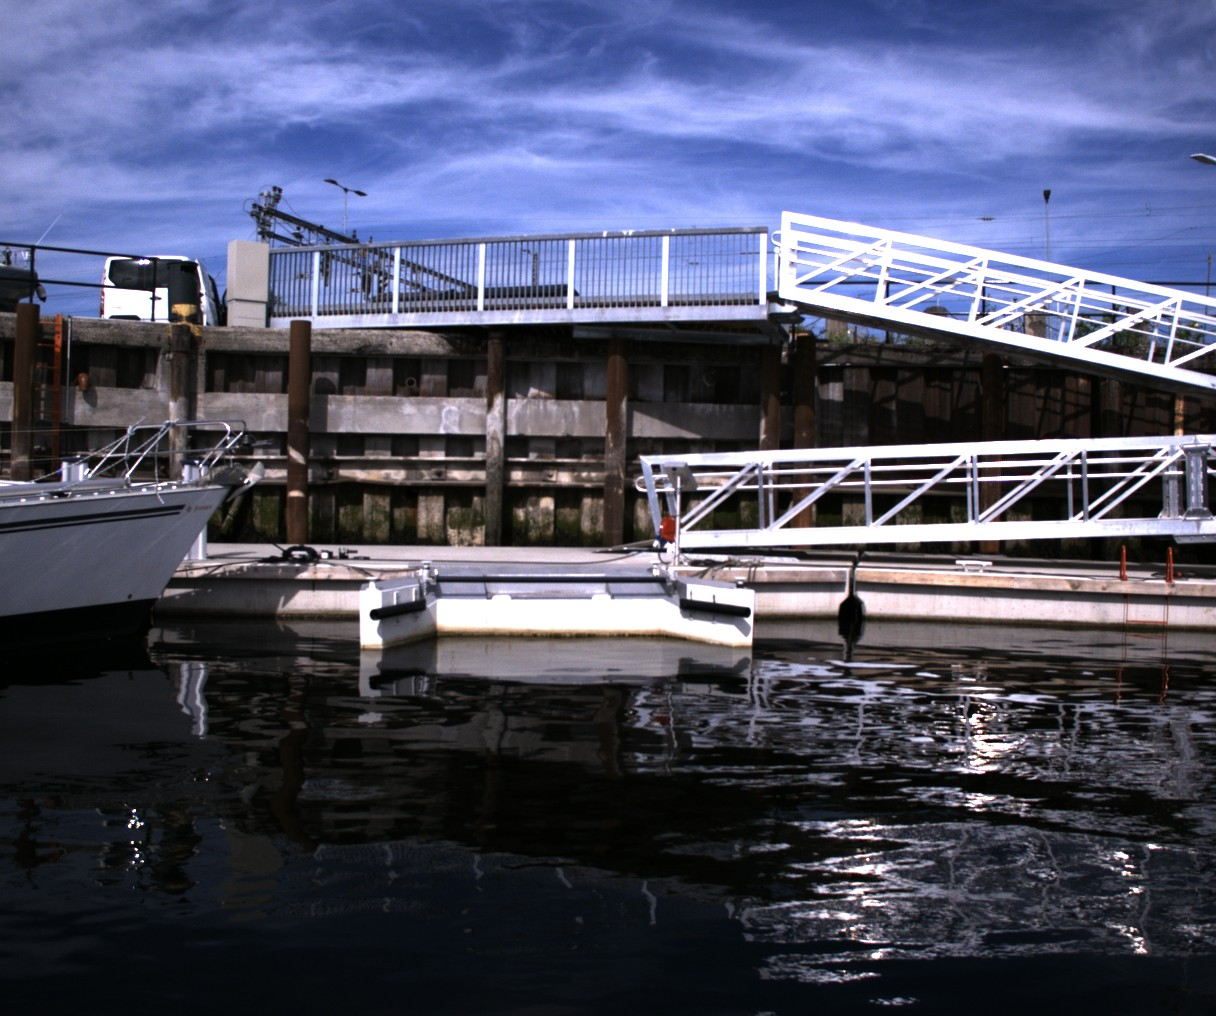
\includegraphics[width=\textwidth]{figures/pictures/img_11640_s0.jpg}
    \end{subfigure} \hfill
    \begin{subfigure}[T]{.49\textwidth}
        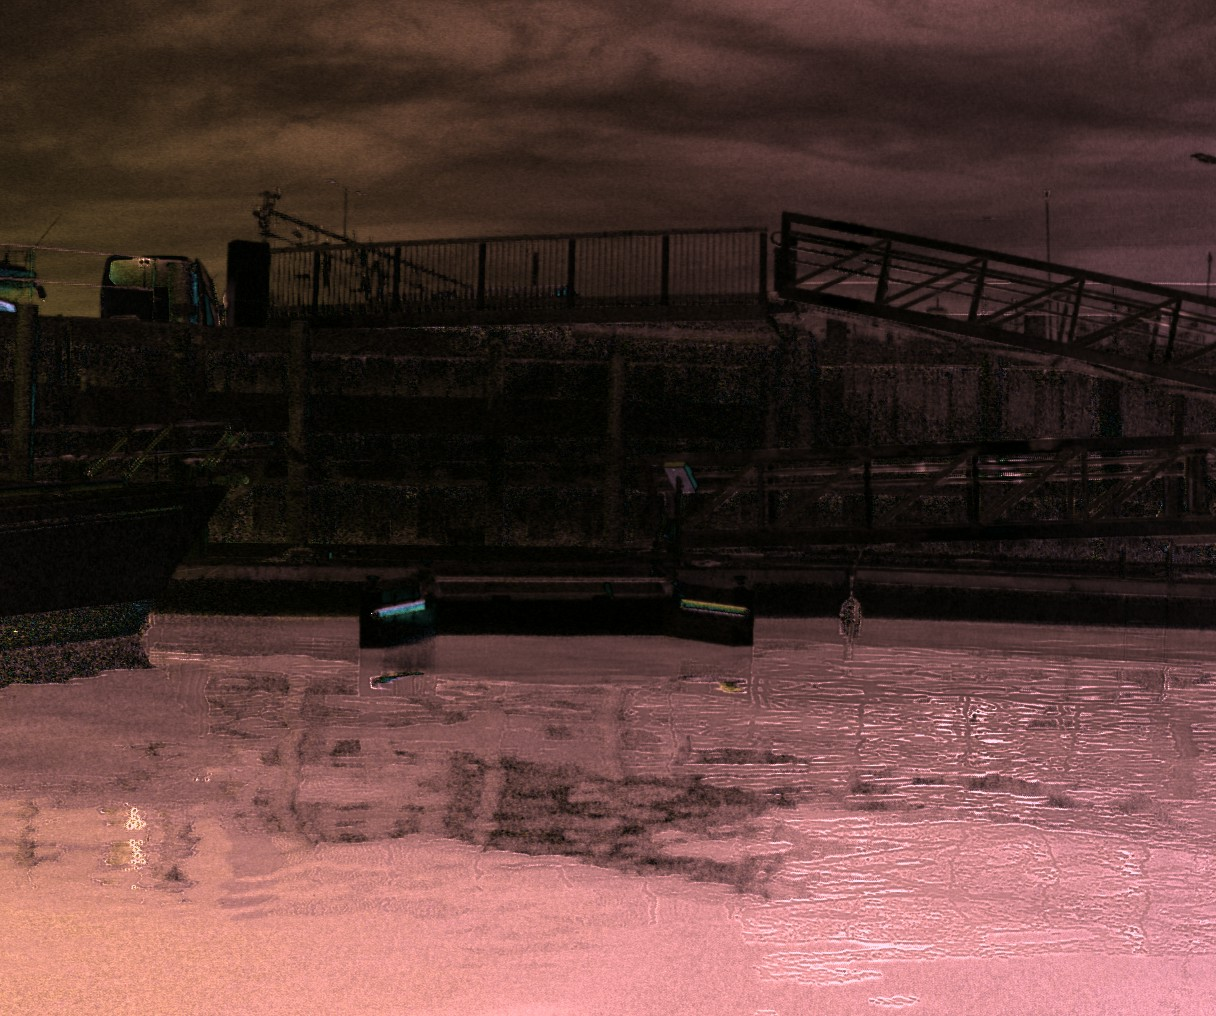
\includegraphics[width=\textwidth]{figures/pictures/img_11640_pol.jpg}
    \end{subfigure}
    \caption{Dock viewed from the water.}
\end{figure}
\vspace{-.5cm}

\begin{figure}[H]
    \begin{subfigure}[T]{.49\textwidth}
        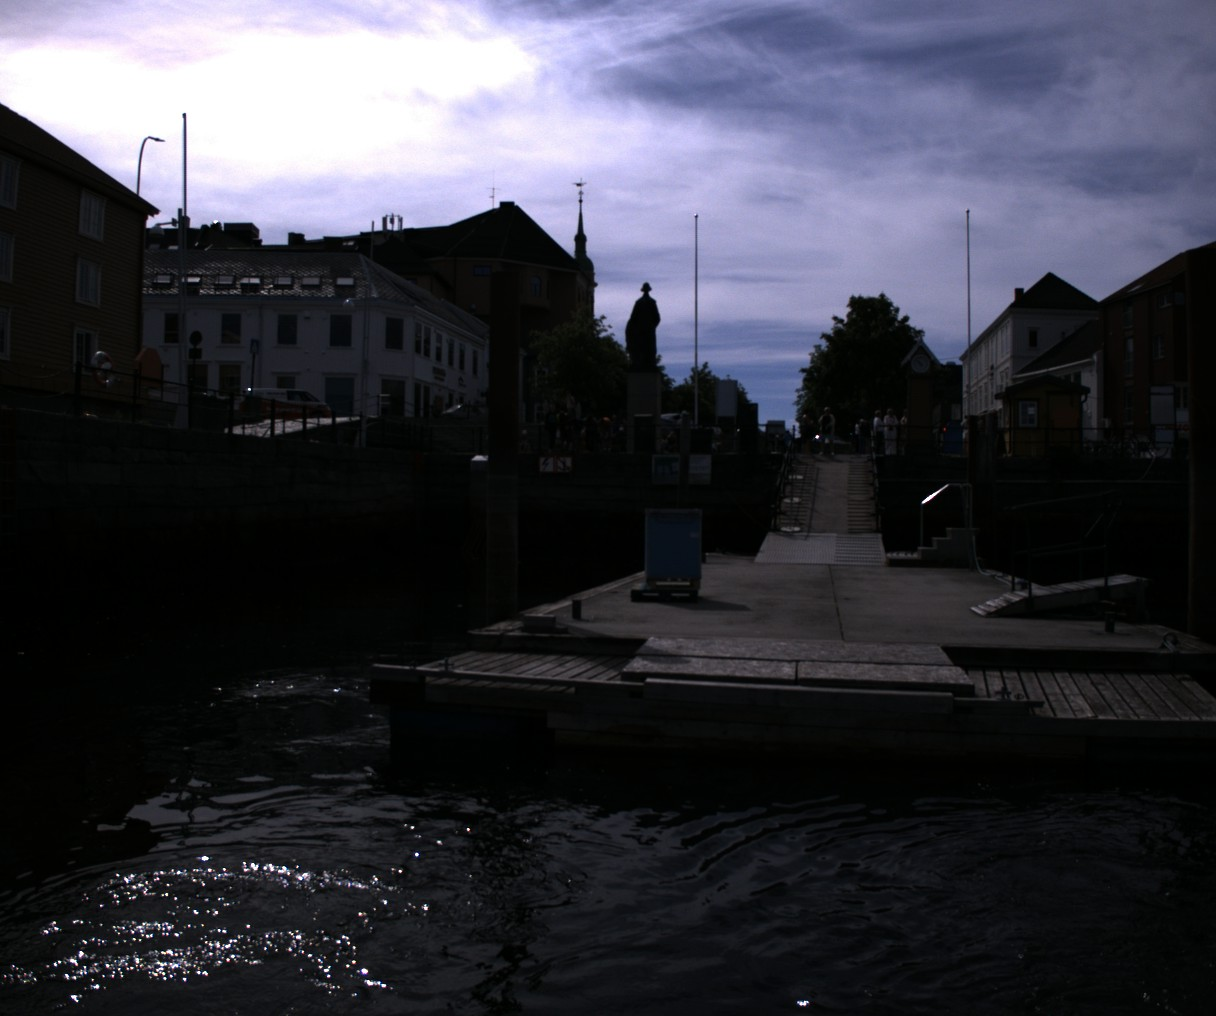
\includegraphics[width=\textwidth]{figures/pictures/img_10170_s0.jpg}
    \end{subfigure} \hfill
    \begin{subfigure}[T]{.49\textwidth}
        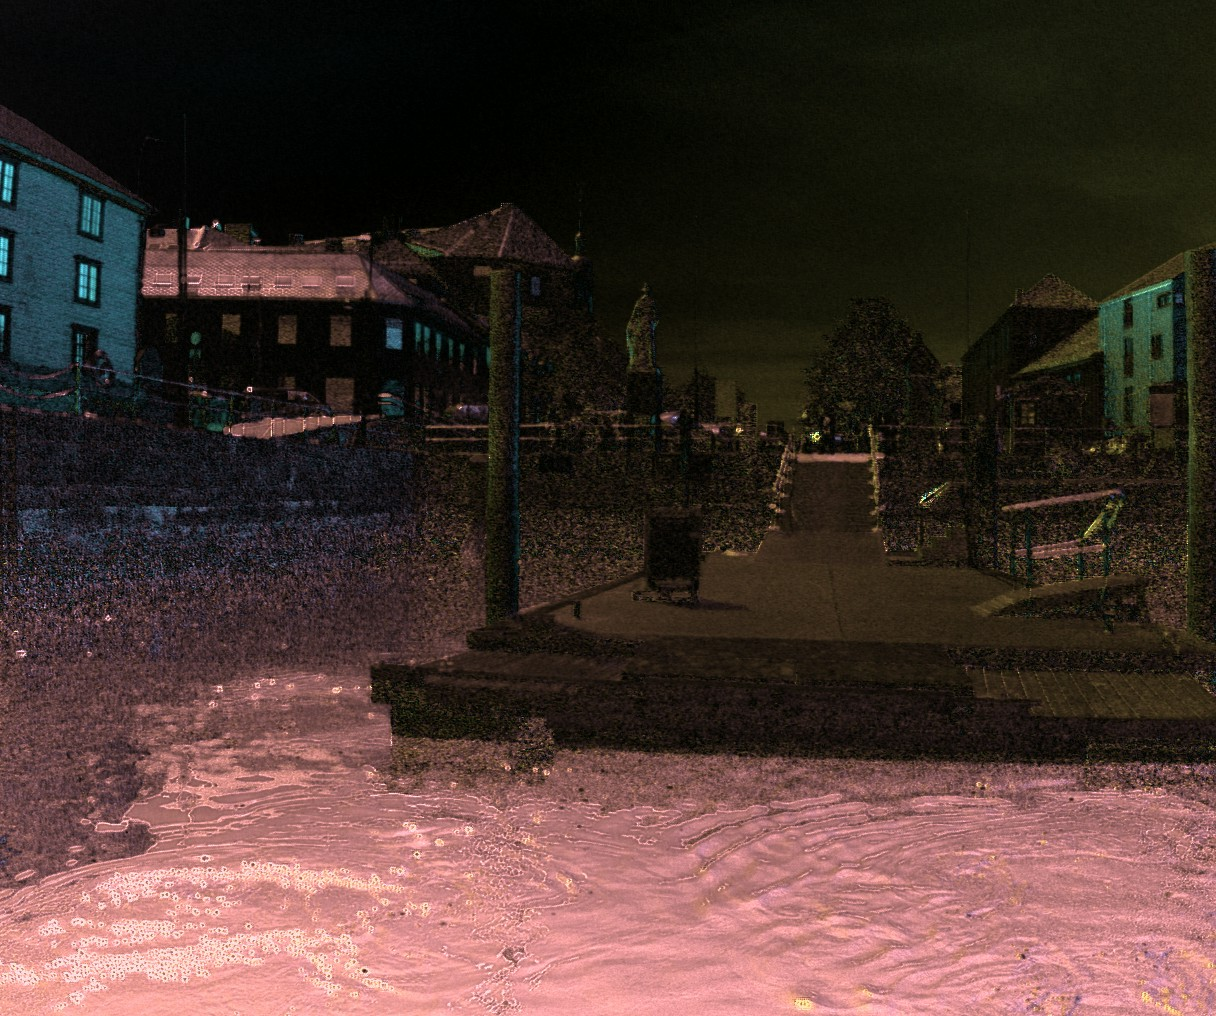
\includegraphics[width=\textwidth]{figures/pictures/img_10170_pol.jpg}
    \end{subfigure}
    \caption{Underexposed image of a dock seen from the water.}
\end{figure}
\vspace{-.5cm}


\begin{figure}[H]
    \begin{subfigure}[T]{.49\textwidth}
        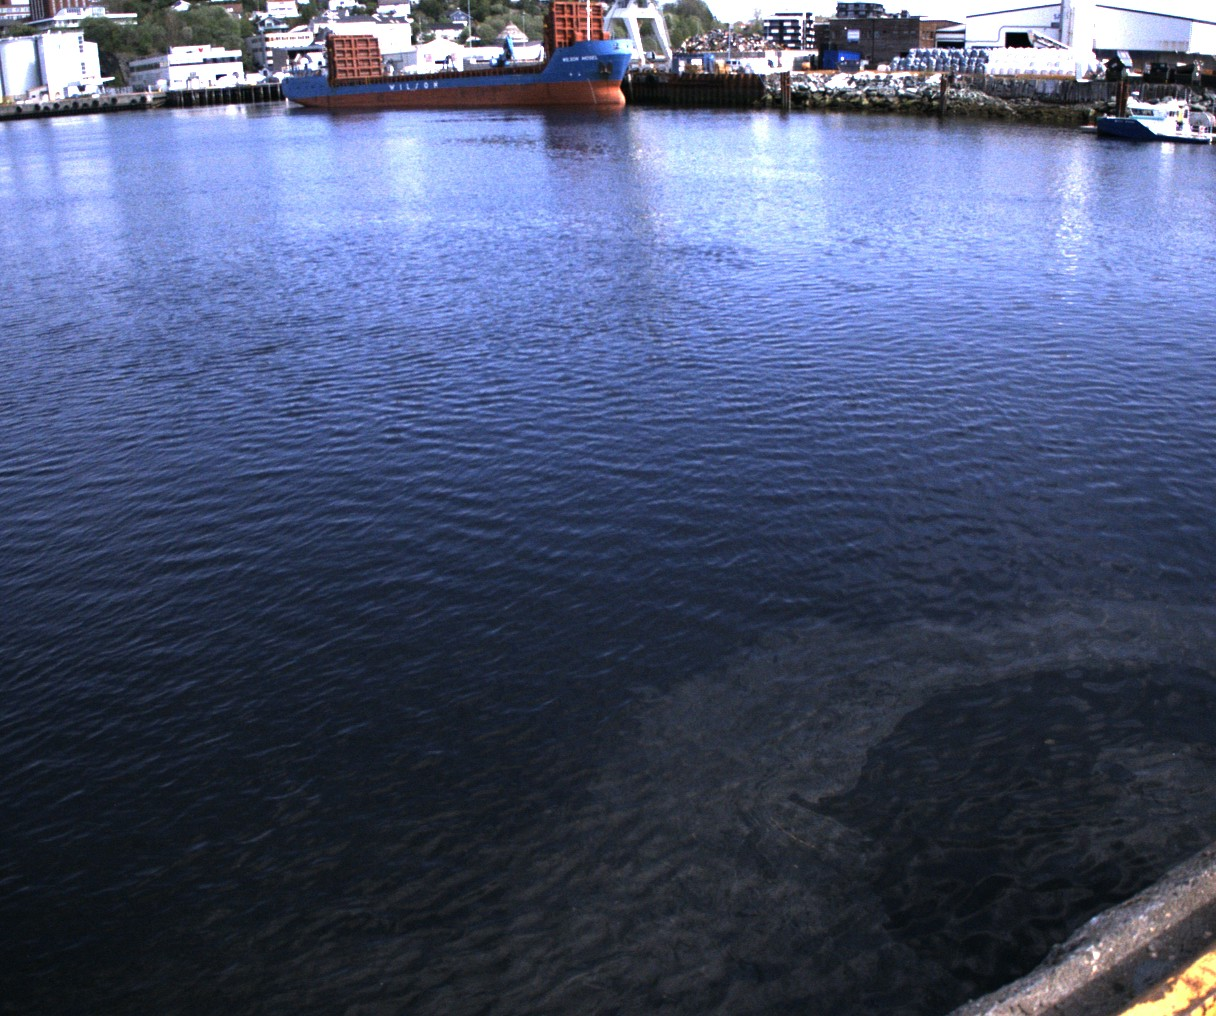
\includegraphics[width=\textwidth]{figures/pictures/img_3726_s0.jpg}
    \end{subfigure} \hfill
    \begin{subfigure}[T]{.49\textwidth}
        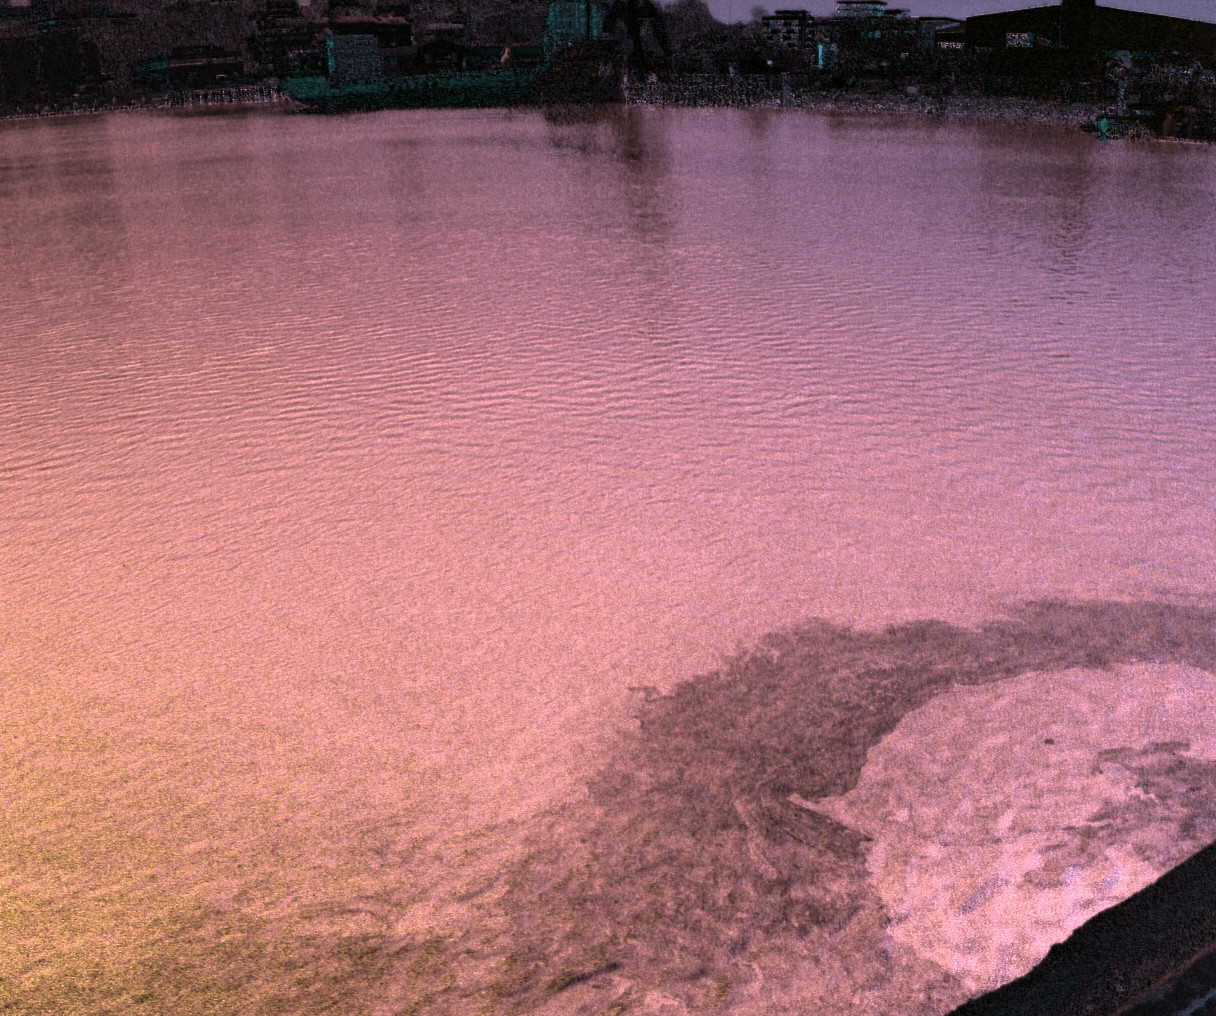
\includegraphics[width=\textwidth]{figures/pictures/img_3726_pol.jpg}
    \end{subfigure}
    \caption{Pollen on the water surface.}
\end{figure}
\vspace{-.5cm}

\begin{figure}[H]
    \begin{subfigure}[T]{.49\textwidth}
        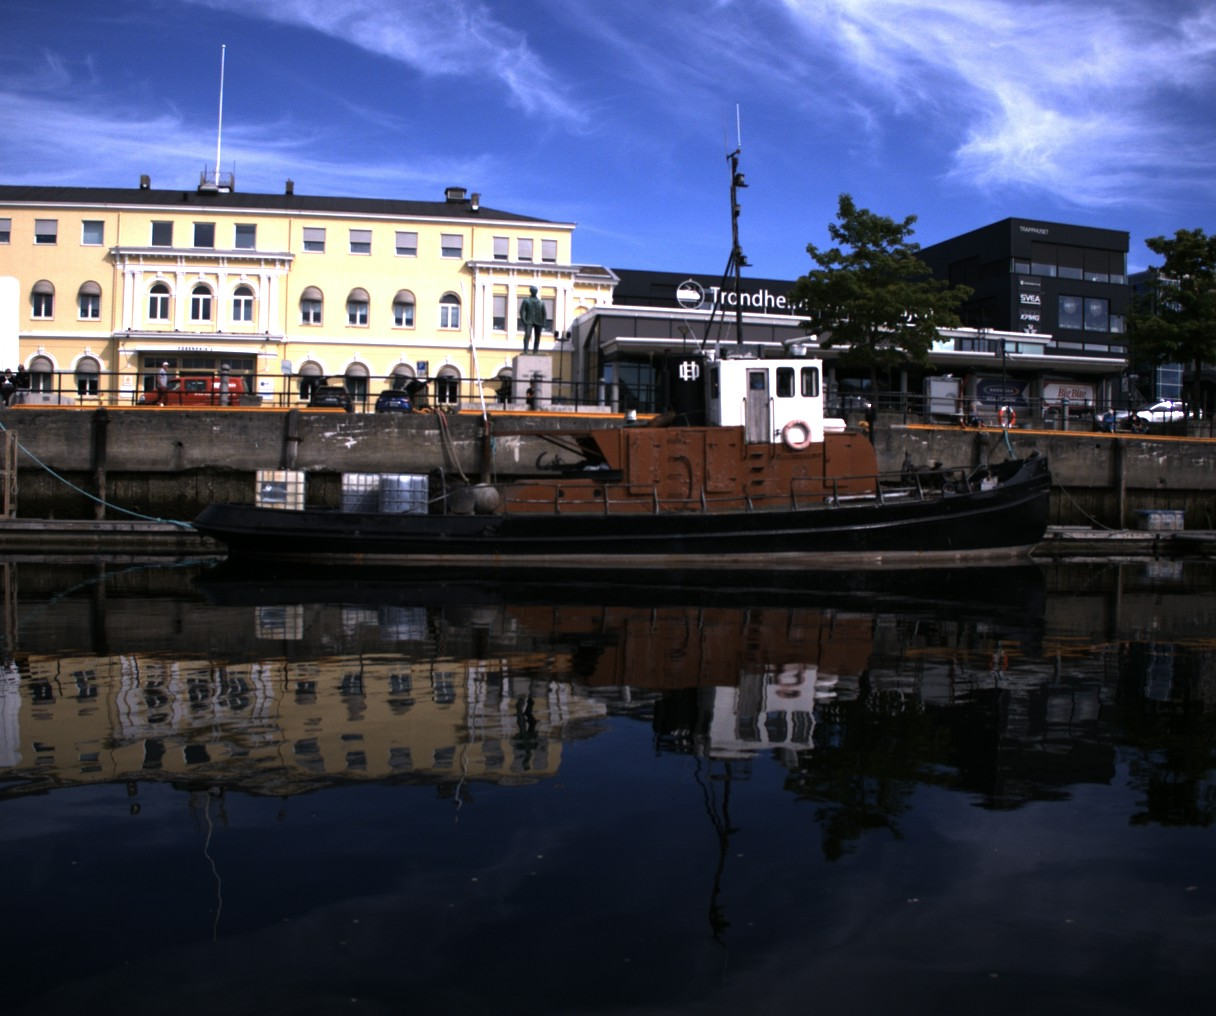
\includegraphics[width=\textwidth]{figures/pictures/img_4038_s0.jpg}
    \end{subfigure} \hfill
    \begin{subfigure}[T]{.49\textwidth}
        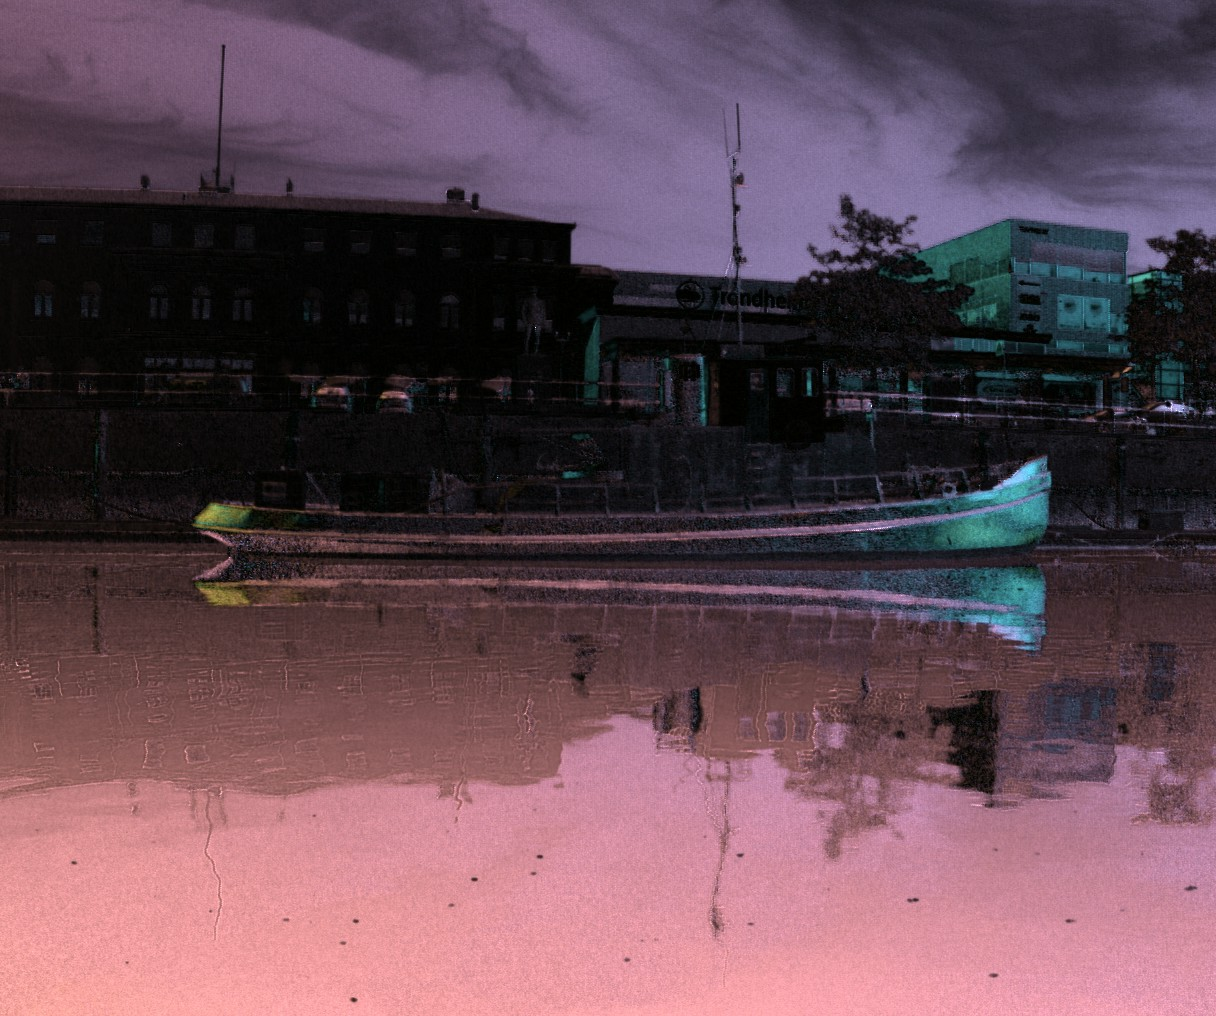
\includegraphics[width=\textwidth]{figures/pictures/img_4038_pol.jpg}
    \end{subfigure}
    \caption{A docked boat seen from the water.}
\end{figure}
\vspace{-.5cm}

% \begin{figure}[H]
%     \begin{subfigure}[T]{.49\textwidth}
%         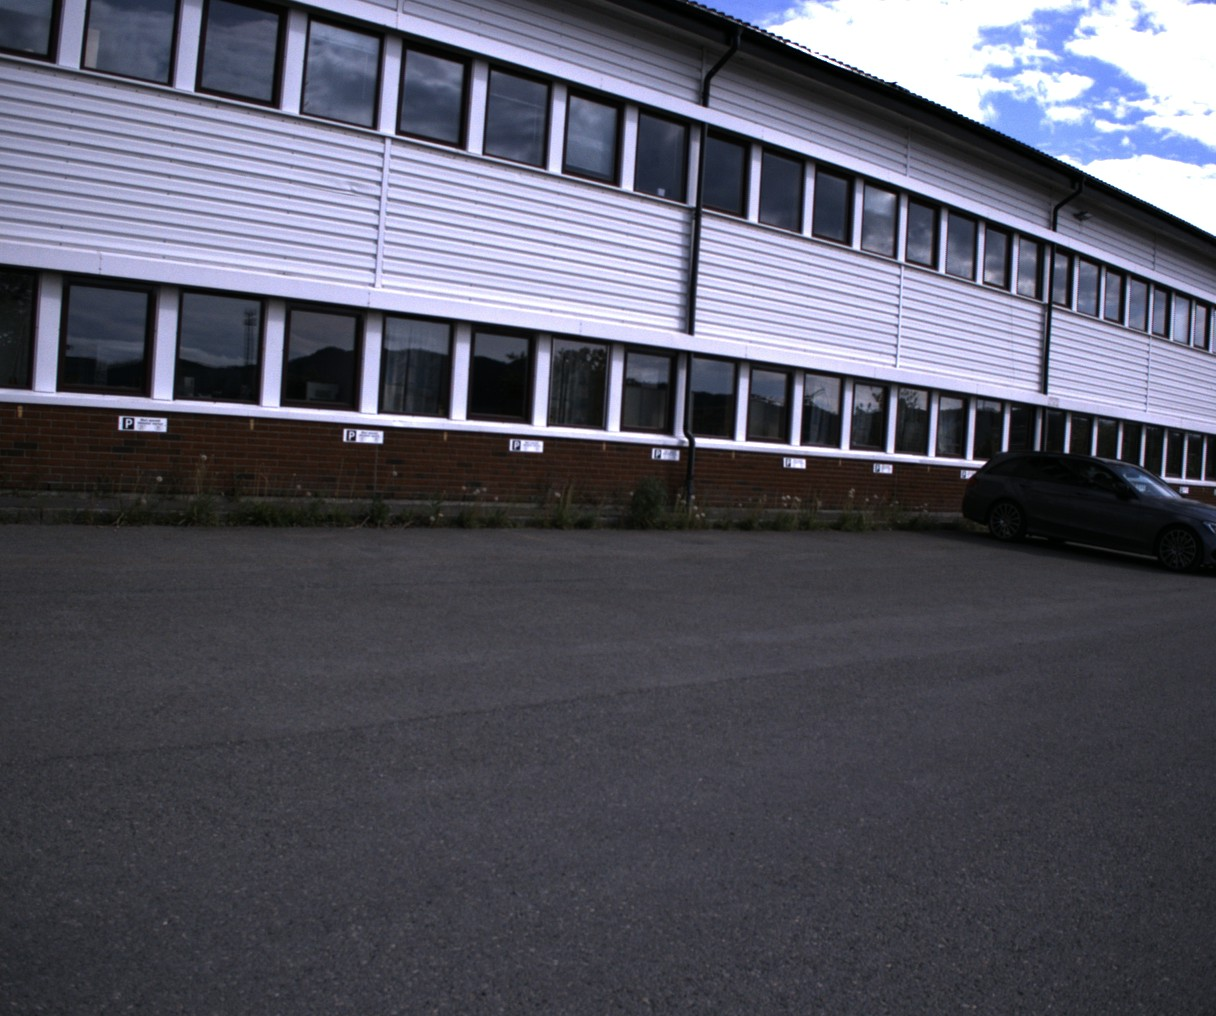
\includegraphics[width=\textwidth]{figures/pictures/img_5742_s0.jpg}
%     \end{subfigure} \hfill
%     \begin{subfigure}[T]{.49\textwidth}
%         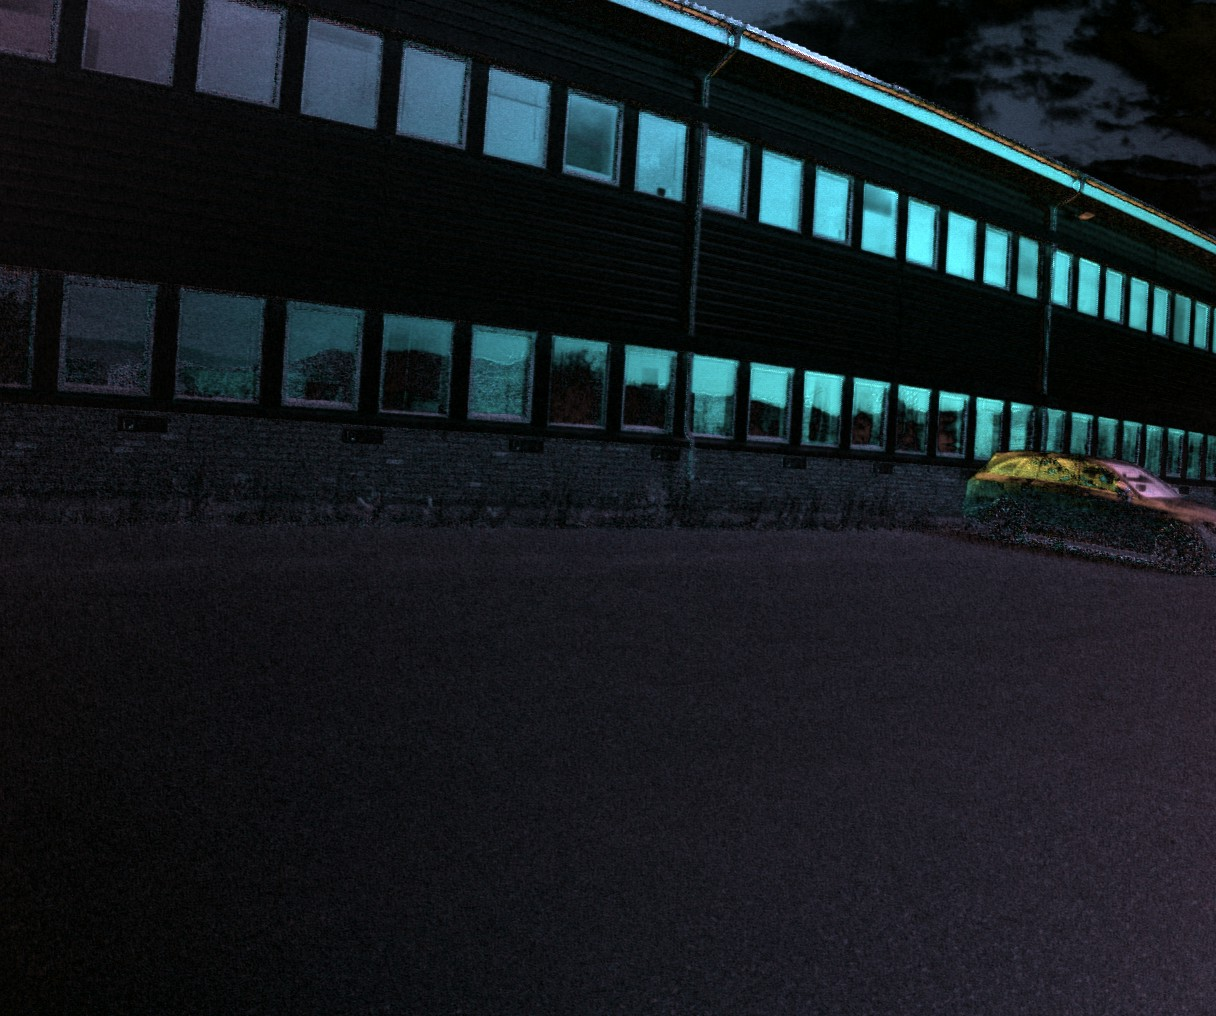
\includegraphics[width=\textwidth]{figures/pictures/img_5742_pol.jpg}
%     \end{subfigure}
%     \caption{Building with glass windows.}
% \end{figure}
% \vspace{-.5cm}
\begin{figure}[H]
    \begin{subfigure}[T]{.49\textwidth}
        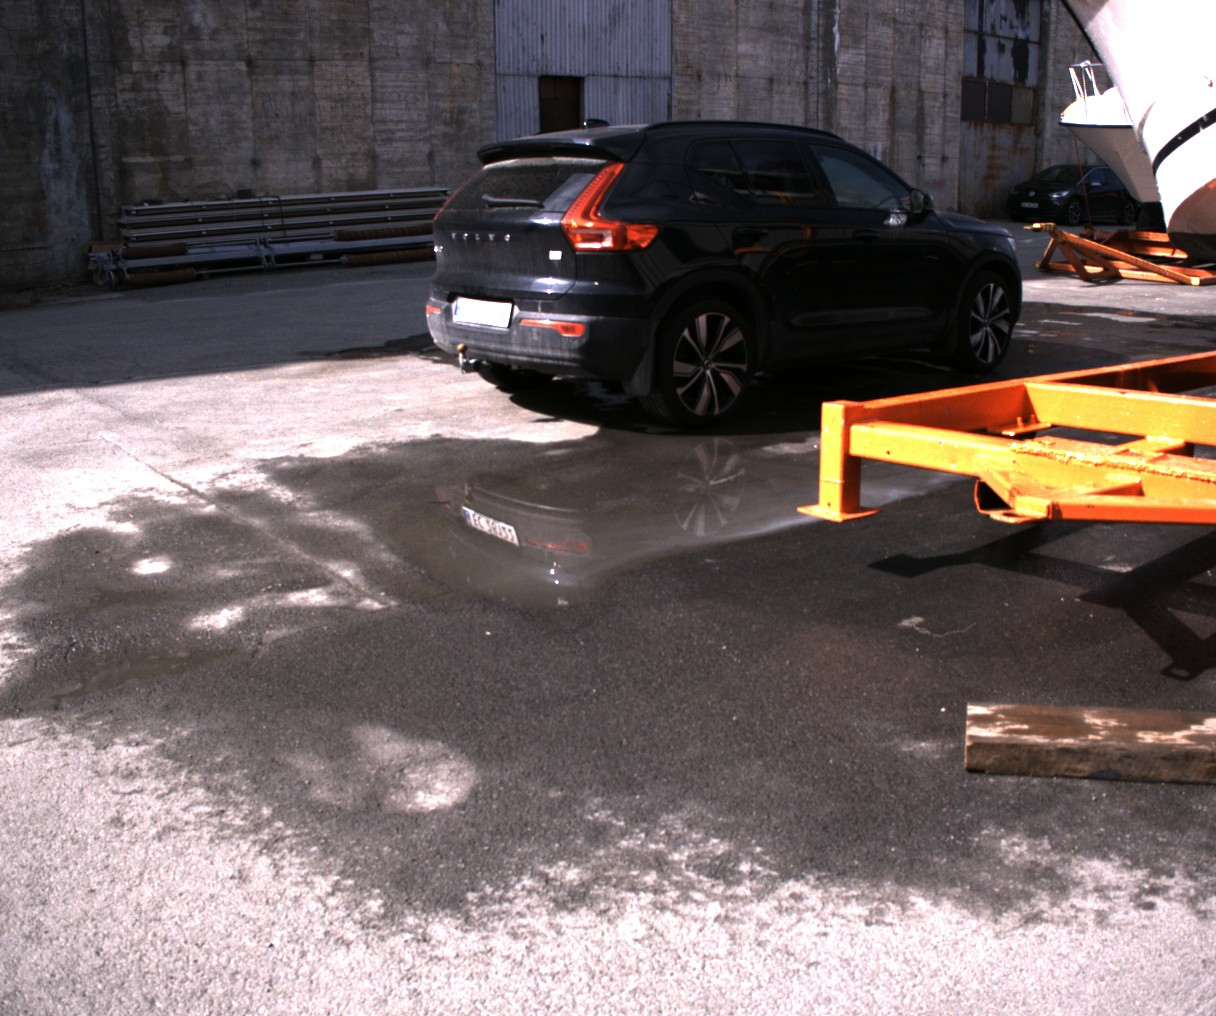
\includegraphics[width=\textwidth]{figures/pictures/img_1116_s0.jpg}
    \end{subfigure} \hfill
    \begin{subfigure}[T]{.49\textwidth}
        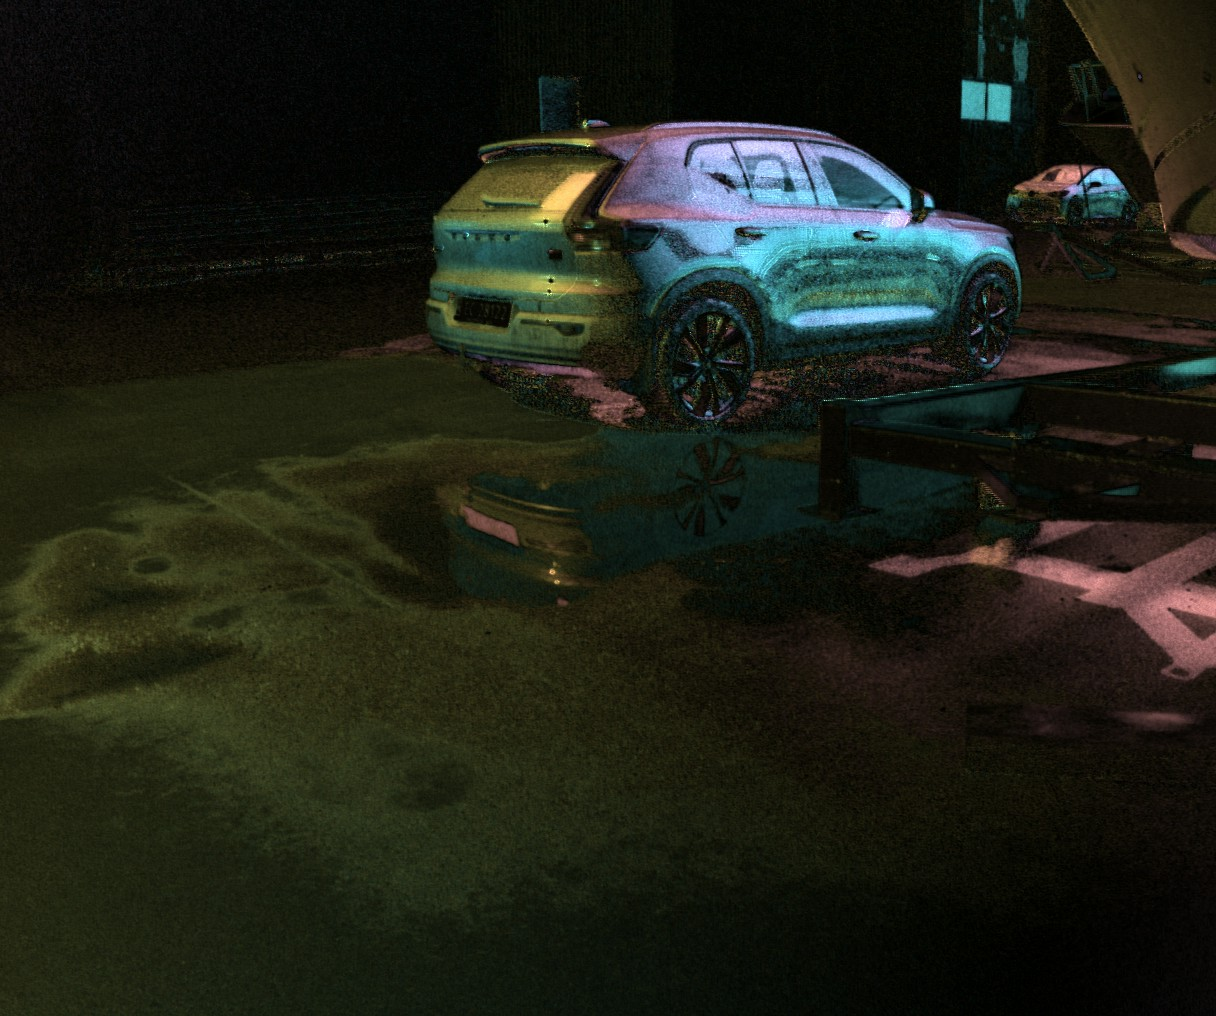
\includegraphics[width=\textwidth]{figures/pictures/img_1116_pol.jpg}
    \end{subfigure}
    \caption{A car standing next to a puddle of water.}
\end{figure}
\vspace{-.5cm}


\begin{figure}[H]
    \begin{subfigure}[T]{.49\textwidth}
        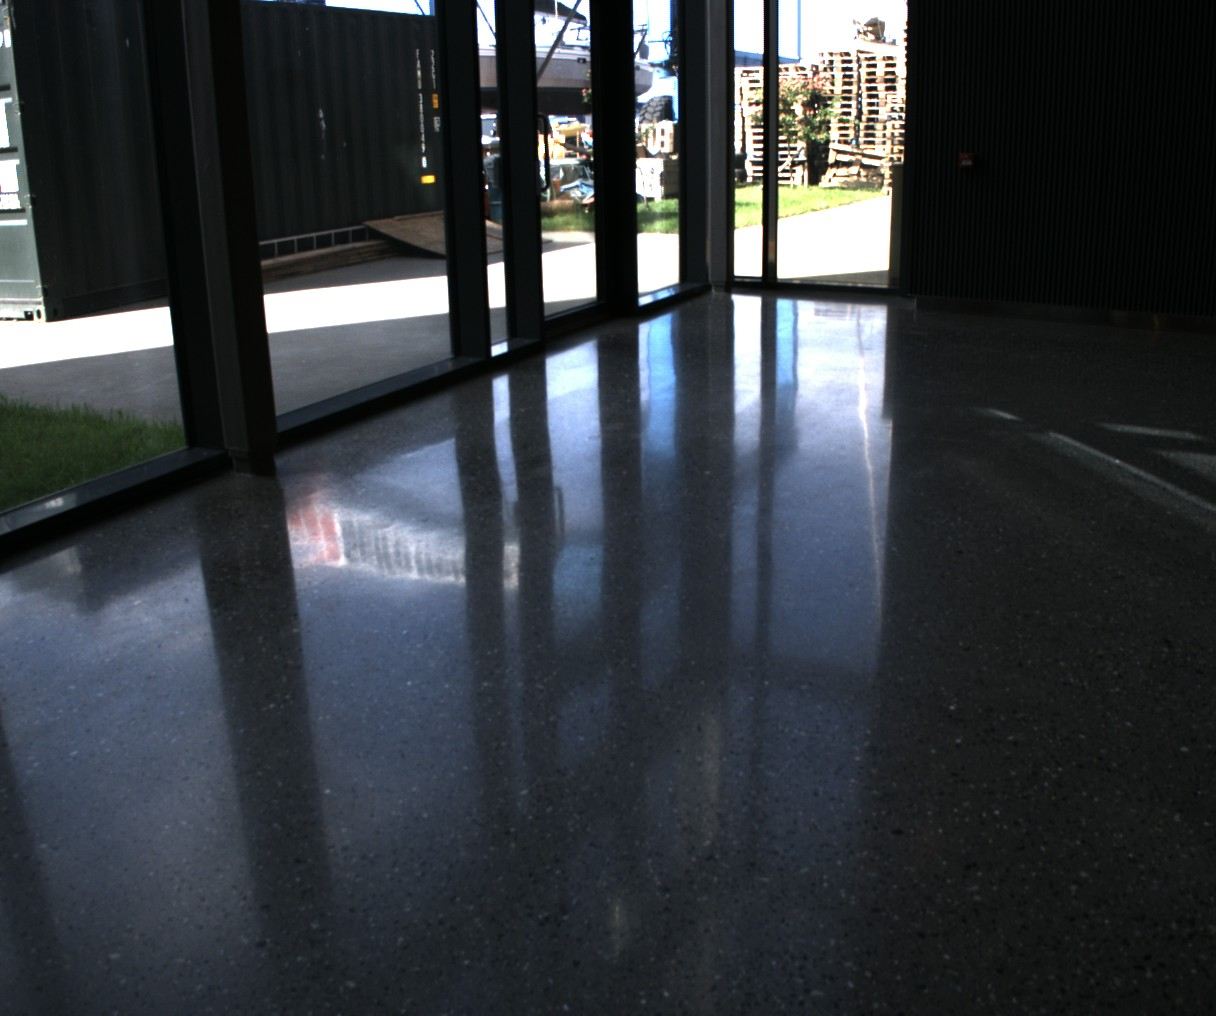
\includegraphics[width=\textwidth]{figures/pictures/img_9222_s0.jpg}
    \end{subfigure} \hfill
    \begin{subfigure}[T]{.49\textwidth}
        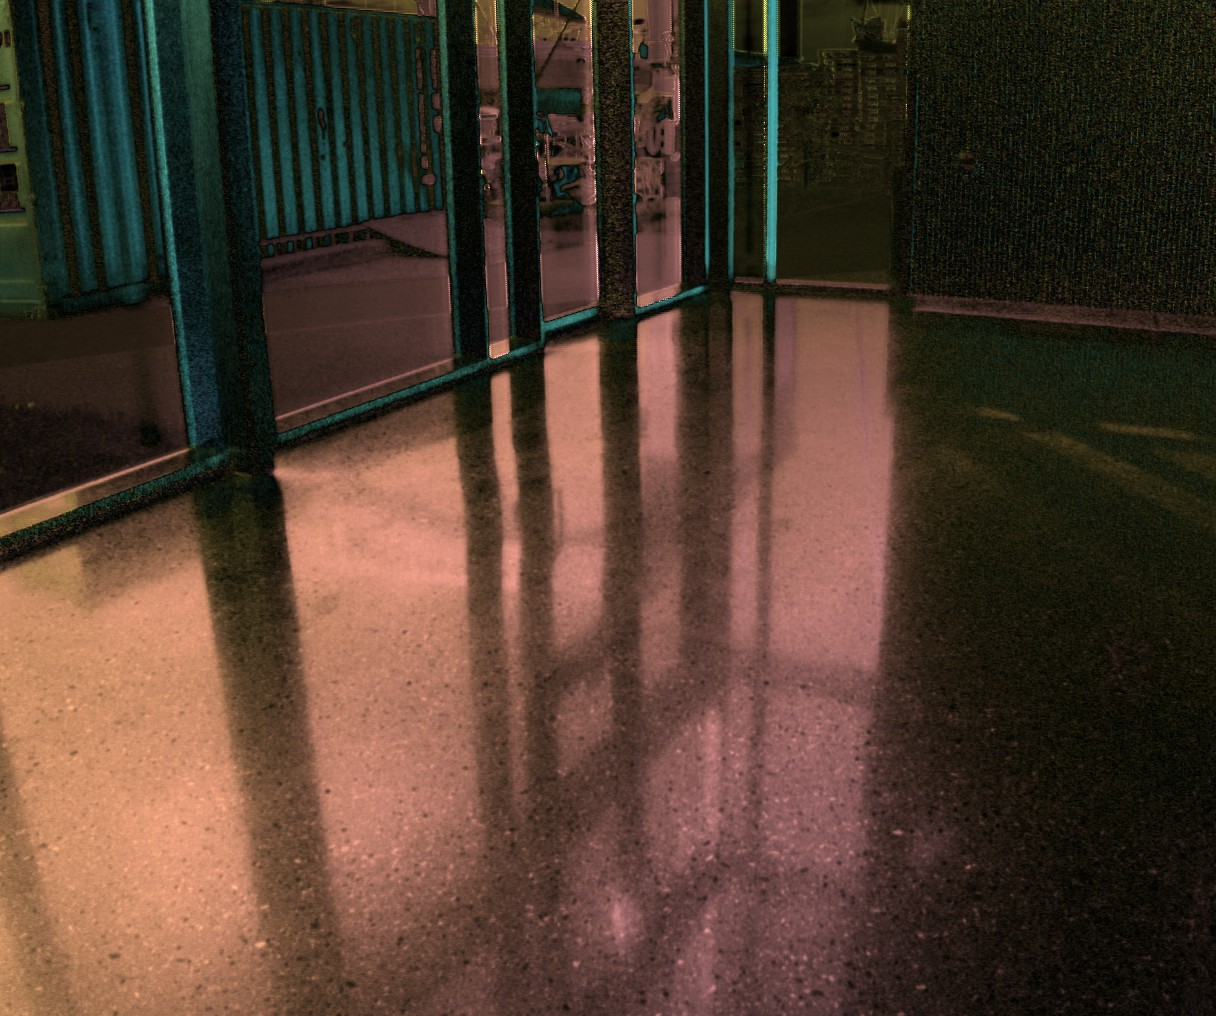
\includegraphics[width=\textwidth]{figures/pictures/img_9222_pol.jpg}
    \end{subfigure}
    \caption{Stone floor with reflections.}
\end{figure}
\vspace{-.5cm}

% \begin{figure}[H]
%     \begin{subfigure}[T]{.49\textwidth}
%         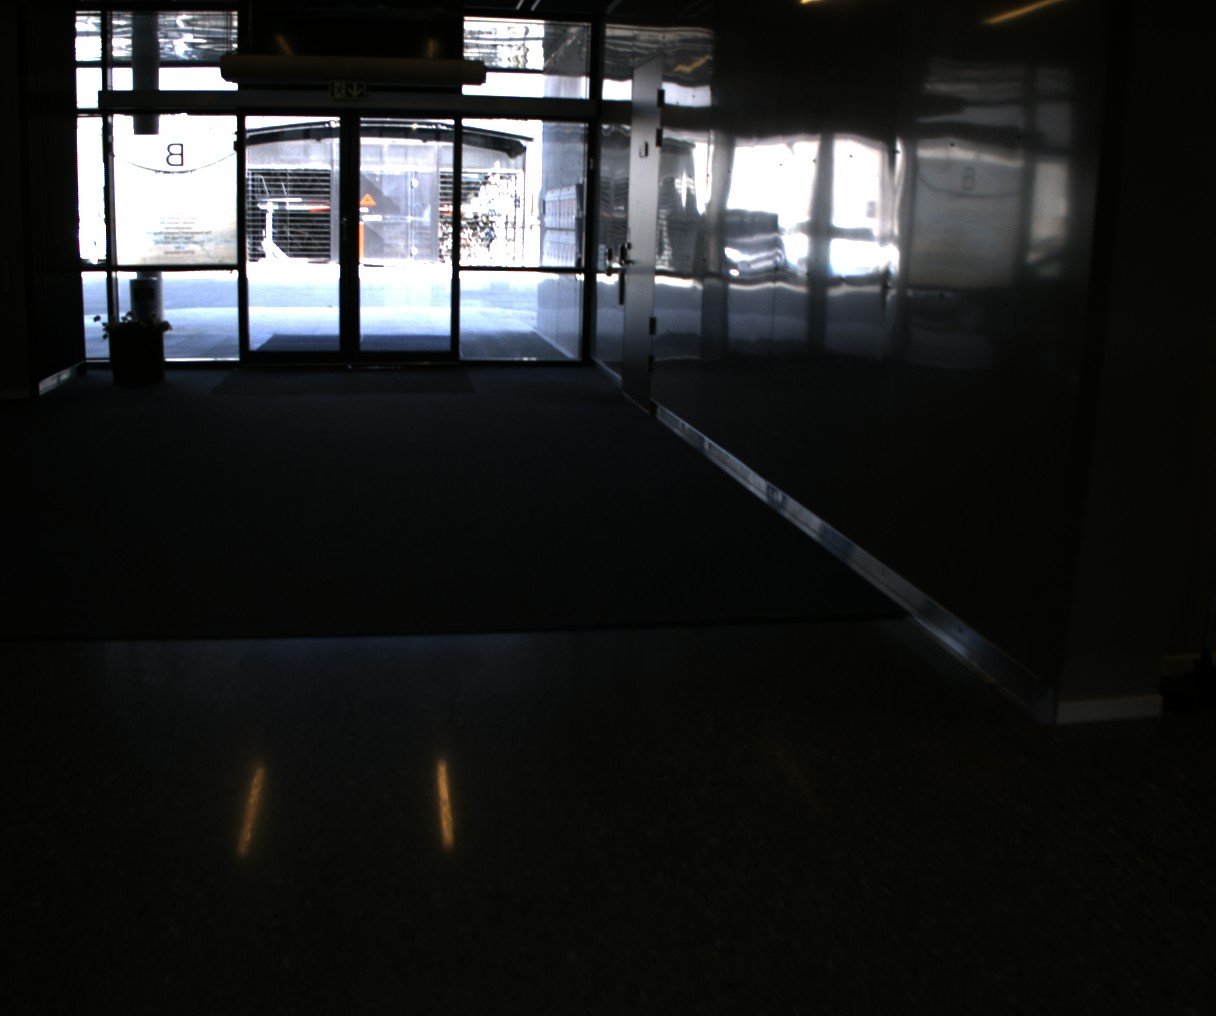
\includegraphics[width=\textwidth]{figures/pictures/img_9306_s0.jpg}
%     \end{subfigure} \hfill
%     \begin{subfigure}[T]{.49\textwidth}
%         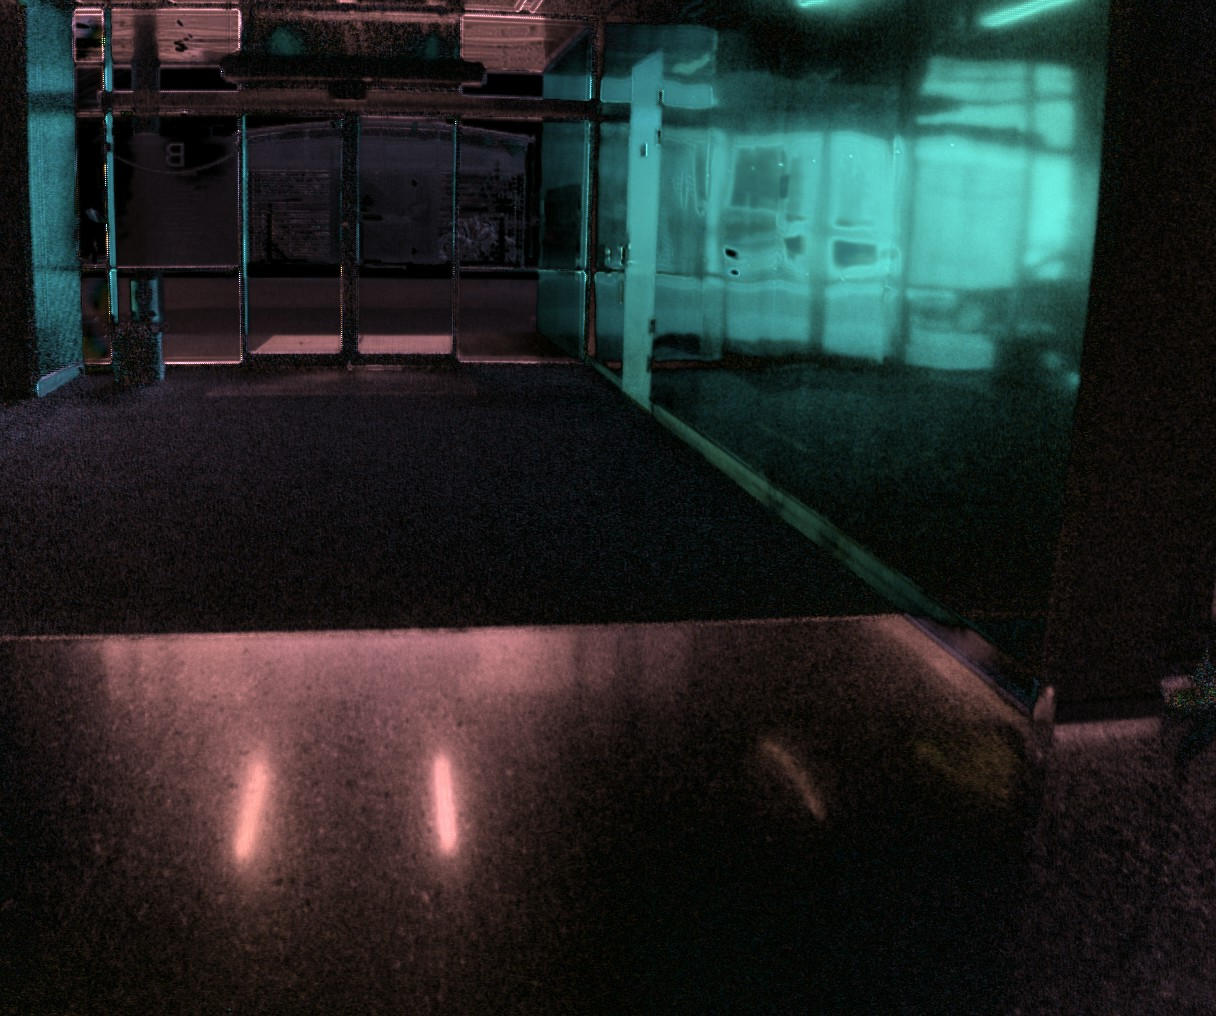
\includegraphics[width=\textwidth]{figures/pictures/img_9306_pol.jpg}
%     \end{subfigure}
%     \caption{High contrast inside environment.}
% \end{figure}
% \vspace{-.5cm}


\begin{figure}[H]
    \begin{subfigure}[T]{.49\textwidth}
        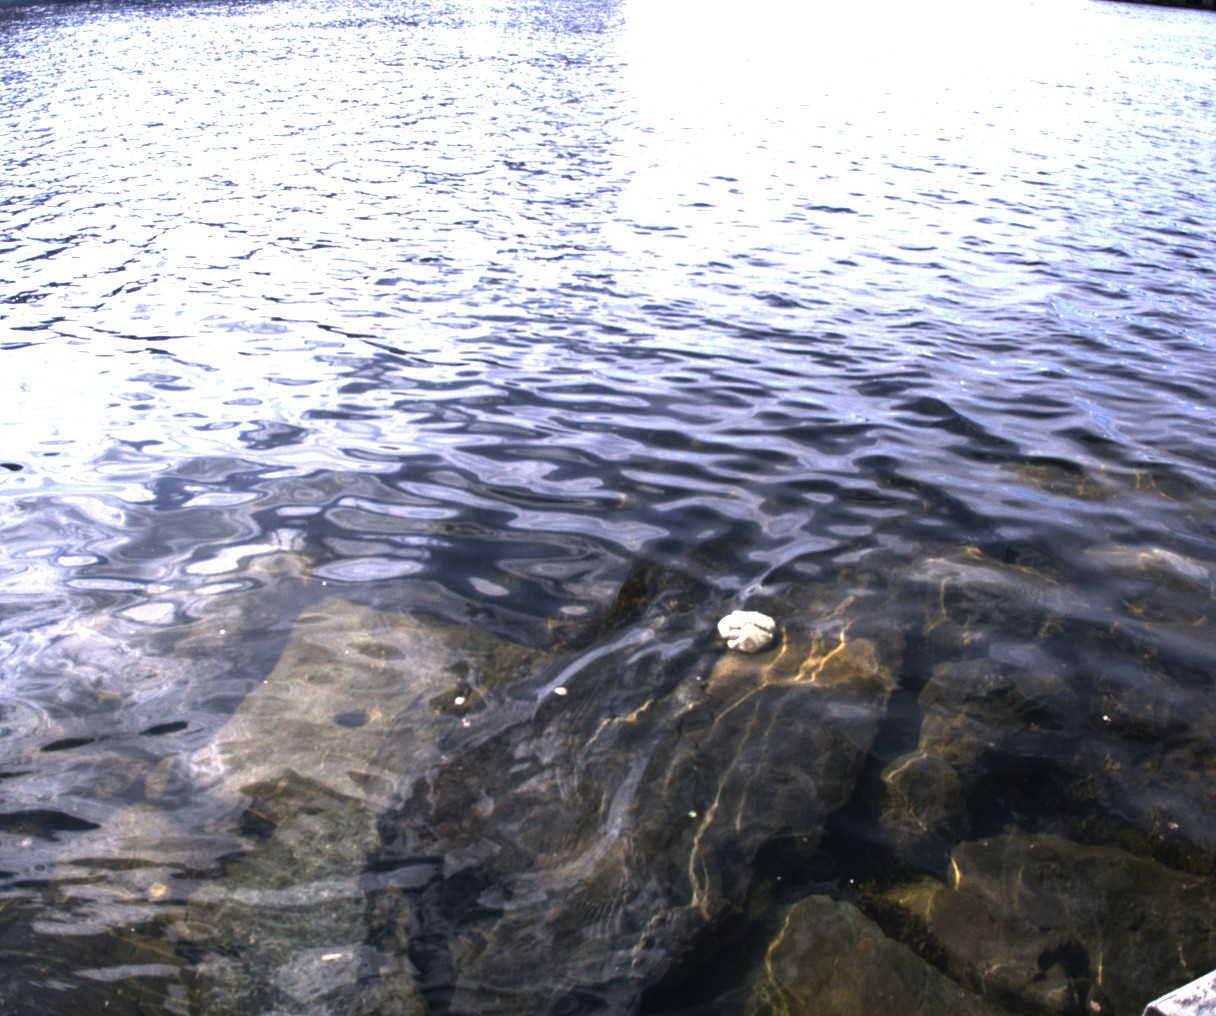
\includegraphics[width=\textwidth]{figures/pictures/img_4722_s0.jpg}
    \end{subfigure} \hfill
    \begin{subfigure}[T]{.49\textwidth}
        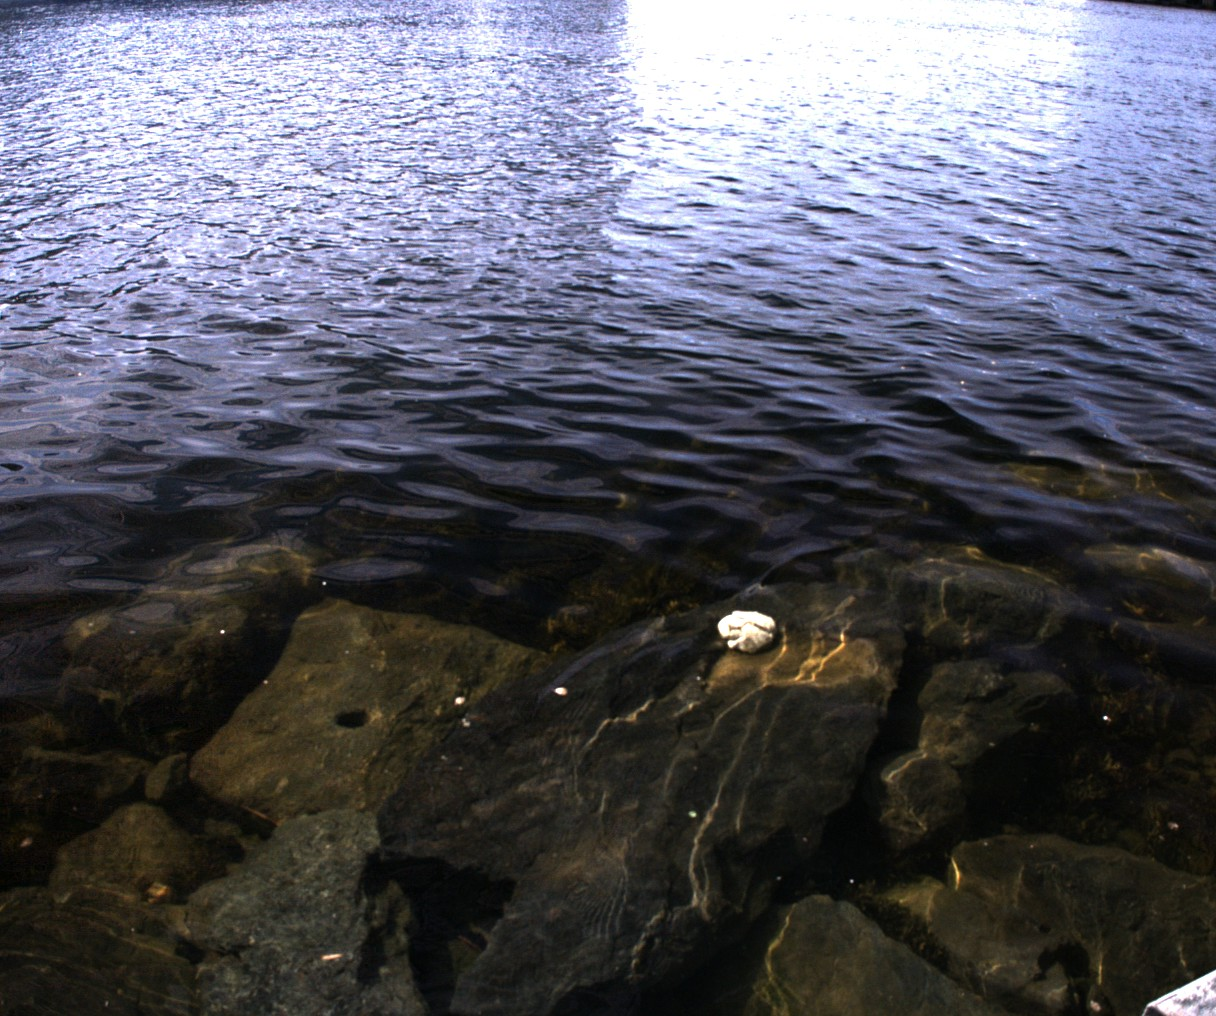
\includegraphics[width=\textwidth]{figures/pictures/img_4722_unpol.jpg}
    \end{subfigure}
    \caption{Image where the linarly polarized light is removed to see whats under the water surface.}
\end{figure}
\vspace{-.5cm}

